\section{Extended Research Notes}
\label{app:research-notes}

This appendix contains additional research notes that support the shorter
research outline in the main report.
They are included here to document the wider Hytale modding landscape
without making the main text too long.

\subsection{Tools and Formats}

Hytale mods are created through a mix of official and semi-official tools.
Important tools include the Hytale Asset Editor,
direct data asset editing,
Blockbench for models and animations,
and Java server plugins for gameplay changes.
These tools suggest that Hytale modding is meant for different kinds of creators:
artists,
builders,
server owners,
and programmers.

Modding is not limited to changing textures or adding small cosmetic details.
It can also involve new systems,
multiplayer rules,
custom items,
and changes to how the game behaves.
This distinction is important for my own project,
because \textit{Trial of the Goddess} is not mainly an asset pack.
It is a Java server plugin that changes rules,
events,
combat values,
and player interactions.

\subsection{Distribution and Community}

The main public distribution platform for Hytale mods is CurseForge.
Public submissions,
collections,
and official contests are organized there,
which makes mods public artifacts that can be shared,
downloaded,
updated,
and discussed by a wider community.

The Hytale modding landscape includes several types of creators:
artists,
programmers,
designers,
server hosts,
toolmakers,
documentation writers,
and community organizers.
Packs are more focused on assets and content,
such as blocks,
mobs,
items,
textures,
models,
and cosmetics.
Plugins are more code-based and can affect commands,
events,
server systems,
minigames,
and deeper gameplay rules.

\subsection{Community Example: Violet's Wardrobe}

One useful example is Violet,
the creator of \textit{Violet's Wardrobe},
a cosmetic mod that adds craftable customization options.
The mod shows the importance of visual and cosmetic creation in Hytale.
Violet is also important as a modder because she later began working with
the Hytale team on official cosmetics.

This shows how modding can become a visible form of creative work
and even a path into the official development process.
In this case,
modding is not only fan activity.
It also becomes a portfolio
and a bridge between community creation and professional development.

\subsection{Development History and Modding Identity}

The modding landscape has also changed because Hytale itself has had an unusual
development history.
The game was announced years ago,
acquired by Riot Games,
cancelled in 2025,
and later revived after the original creators reacquired it.
Reporting on the revival emphasized that Hytale's return was connected to its
original creator-focused vision and modding support from day one.

Hytale is therefore not only a game that allows mods.
It is a game whose public image and future are strongly tied to the promise
of community creation.

\subsection{Experimental Modding}

Early Hytale modding also shows how unpredictable creator communities can be.
Shortly after launch,
players created experimental mods that ran Windows 95,
Minecraft,
and even Hytale itself inside Hytale.
These are not typical gameplay mods,
but they show that strong modding tools can turn a game into a platform
for unexpected experiments.

This is one reason why Hytale is useful for a critical modding project.
It shows modding becoming part of the development pipeline:
mods are created with official tools,
shared through public platforms,
used to build multiplayer spaces,
and sometimes recognized by the developers themselves.


\section{Dialogue Variants}
\label{app:dialogue}

This appendix contains additional dialogue states used by the Goddess statue.

\subsection{Refusing the Trial}

\begin{tcolorbox}[
    title={Refusing the trial},
    colback=gray!5,
    colframe=gray!60,
    arc=2mm,
    boxrule=0.5pt
]
    Then leave me to my silence.

    \medskip

    \textit{The stone grows cold beneath your hand.}
\end{tcolorbox}

\subsection{Returning without the Sacred Flower}

\begin{tcolorbox}[
    title={Returning without the Sacred Flower},
    colback=gray!5,
    colframe=gray!60,
    arc=2mm,
    boxrule=0.5pt
]
    The Sacred Flower is not with you.

    \medskip

    Find it and bring it to me...

    \medskip

    So I can be complete once again.
\end{tcolorbox}

\subsection{Completing the Trial}

\begin{tcolorbox}[
    title={Completing the trial},
    colback=gray!5,
    colframe=gray!60,
    arc=2mm,
    boxrule=0.5pt
]
    \textit{The Sacred Flower trembles in your hands.
    Its light sinks into the cold stone.}

    \medskip

    Finally... I am whole again.

    \medskip

    Thank you,
    little wanderer.

    \medskip

    I have no need for the blade anymore.

    \medskip

    Keep it,
    as a sign of my gratitude.

    \medskip

    Now... I may slumber.
    Farewell...

    \medskip

    \textit{The warmth fades.
    The voice is gone.
    The statue is only stone again.}

    \medskip

    \textit{The Trial of the Goddess is complete.}
\end{tcolorbox}




\section{Technical Documentation}
\label{app:implementation-details}

This appendix contains the detailed implementation notes that support the
shorter overview in the main report.

\subsection{Full Dependency Graph}

\begin{center}
    \includegraphics[width=0.95\textwidth]{images/mermaid-diagram-even-more-confusing}

    \small
    Figure: Full dependency graph generated from the source code.
    The graph is intentionally dense and shows the implementation complexity
    behind a seemingly simple gameplay loop.
\end{center}



\subsection{Simplified Architecture}

The full dependency graph is useful as evidence of complexity,
but it is too detailed to explain the mod clearly.
The simplified architecture groups the plugin into six responsibilities:
assets,
entry points,
trial state,
gameplay systems,
player feedback,
and cleanup.
These responsibilities make the mod feel like one continuous ritual
while keeping the code separated into smaller systems.

\begin{center}
    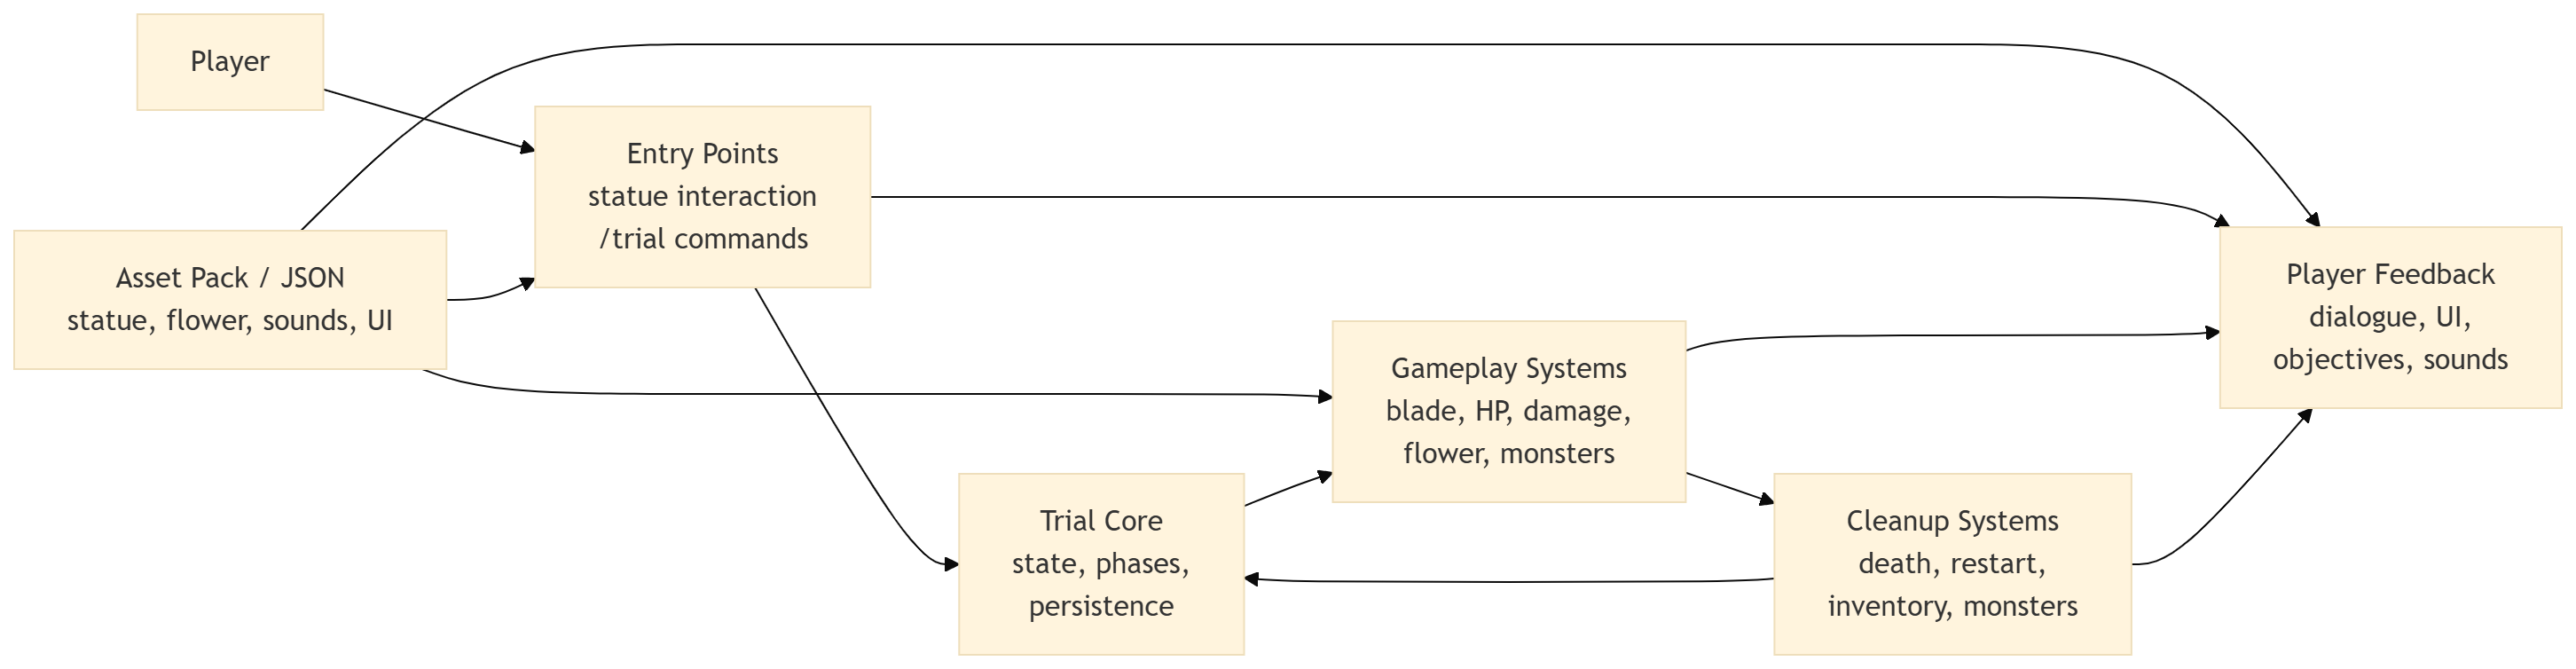
\includegraphics[width=0.95\textwidth]{images/mermaid-abstact}

    \small
    Figure: Simplified architecture of the GoddessTrial plugin.
    The diagram groups the implementation into the main responsibilities
    instead of showing every class and dependency.
\end{center}


\subsection{Asset Pack and JSON Configuration}

The asset layer was originally planned as a supporting part of the mod.
I expected the main logic to happen in Java,
while assets would only provide the statue,
the Blade of Balance,
the Sacred Flower,
and the sound effects.
This turned out to be too simple.
In Hytale,
not every block automatically creates an interaction event.
The Goddess statue only became usable after its JSON configuration was changed
to point to the custom \texttt{GoddessTrial\_Statue} interaction.

This made asset files part of the actual implementation logic.
To find the right structure,
I had to inspect existing Hytale JSON files
and compare the statue to other interactive blocks.
The same happened with the Sacred Flower.
At first,
the plugin only remembered the position of an ordinary flower
and treated that position as special.
The final version uses a custom Sacred Flower asset with its own item/block ID,
quest tags,
a purple texture,
and a light property that makes it glow.
The objective is therefore visible in the world,
not only hidden in Java state.

One unresolved asset issue remains:
the Sacred Flower appears correctly in the world,
but the inventory displays its internal item ID
instead of the name from the language file.
I could not determine whether this was caused by the language file path,
the translation key,
or Hytale's current asset loading behavior.
Since it does not affect the trial logic,
I left it as a minor visual bug.

The asset layer therefore does more than provide visuals.
It defines which objects can be interacted with,
which items and sounds exist,
where the flower can spawn,
and how the player recognizes the objective.


\subsection{Entry Points}

The mod has two entry points:
the Goddess statue and the \texttt{/trial} commands.
The commands were mainly useful during development,
because they allowed me to test starting,
accepting,
refusing,
resetting,
and checking the trial before the statue interaction worked reliably.
In the final mod,
the statue is the main player-facing entry point,
while the commands remain as debugging and recovery tools.

The main challenge was that the same statue interaction had to mean different things
depending on the current situation.
It can start the prayer sequence,
skip already-running dialogue,
remind the player to find the flower,
complete the ritual,
or remain silent after the Goddess is gone.
The statue therefore became a state-dependent gateway rather than a simple button.

This also required persistent storage.
A completed trial must survive disconnects and restarts,
otherwise the Goddess could offer the ritual again.
Unfinished trials,
however,
are not restored after a restart.
This was a deliberate simplification:
restoring active trials created unstable cases with old items,
leftover flowers,
monsters,
and health effects.
Instead,
unfinished trials are treated as failed and cleaned up when the player returns.


\subsection{Trial Core}

The Trial Core is the rule system behind the ritual.
It decides which actions are valid at which moment,
while other systems create the visible effects.
The trial behaves like a small state machine:
the player moves from no trial,
to an offered trial,
to an active trial,
and finally either back to no trial after failure
or into the permanent completed state.

This shared state prevents different parts of the mod from contradicting each other.
The statue,
commands,
UI buttons,
death handling,
flower pickup,
and cleanup systems all depend on the same trial phase.
Without this shared source of truth,
the player could accept a trial that was never offered,
complete a trial that is not active,
or restart the ritual after it has already been completed.

\begin{center}
    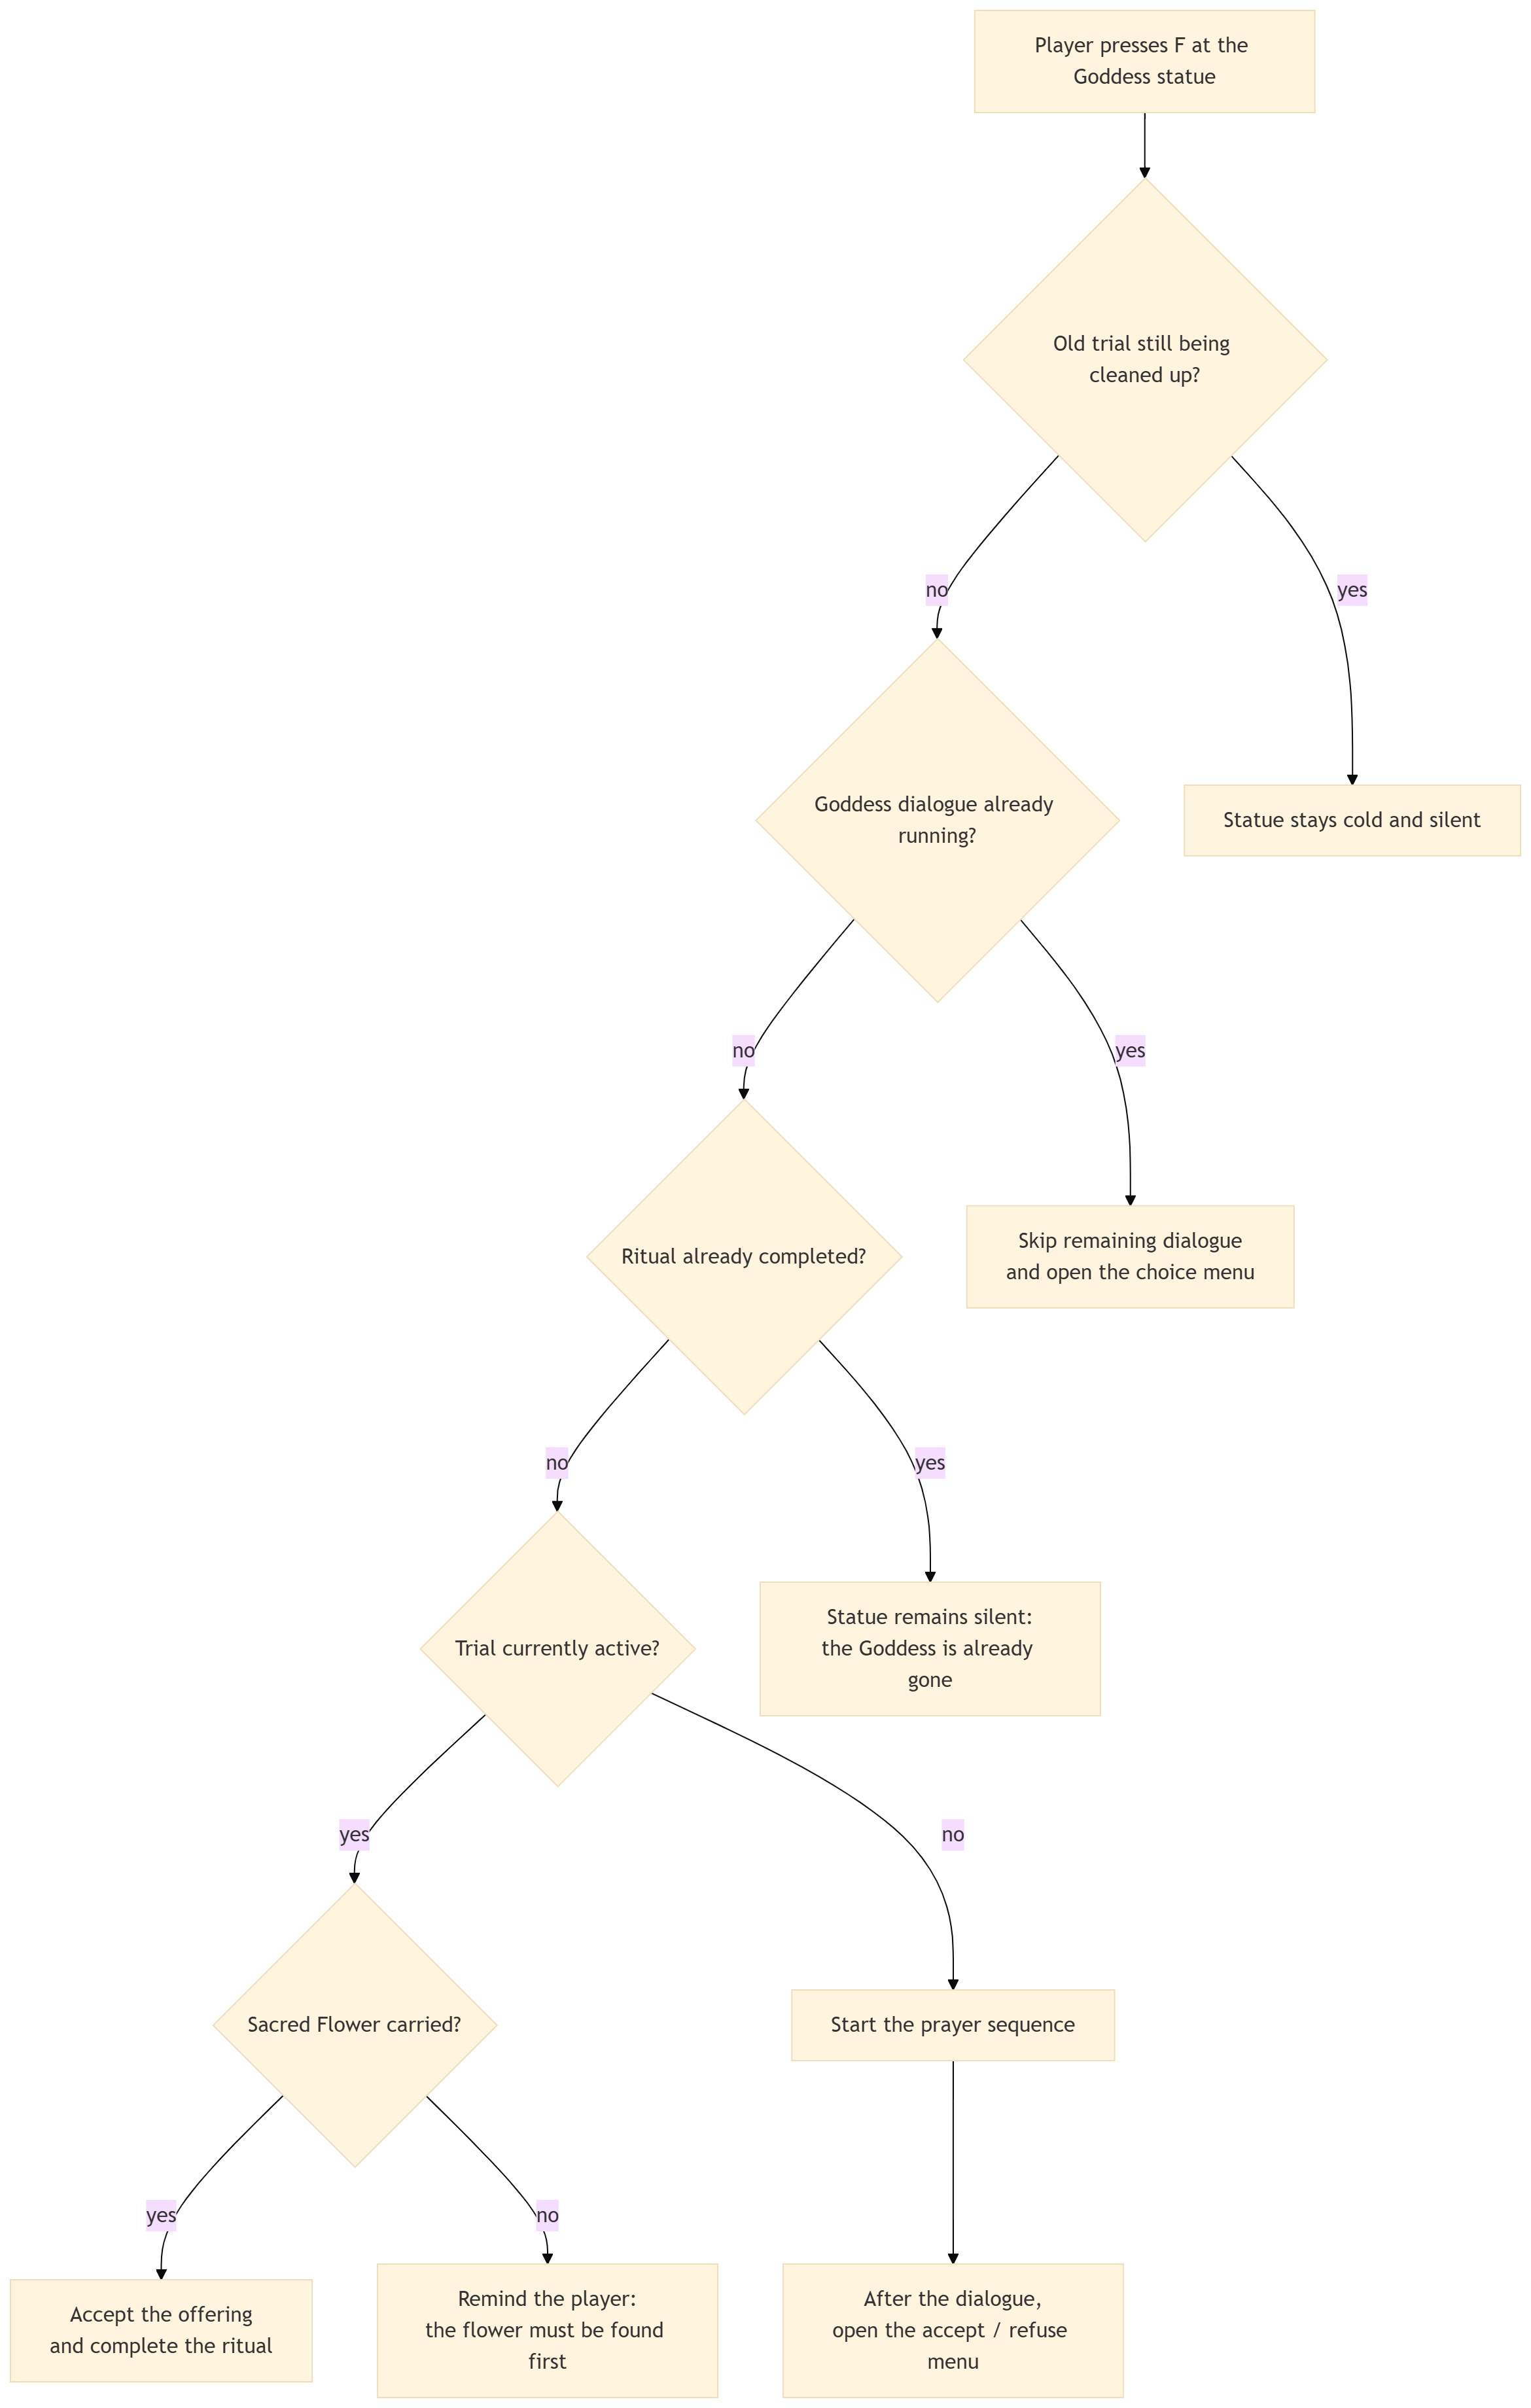
\includegraphics[height=0.55\textheight,keepaspectratio]{images/statuelogic}

    \small
    Figure: State-dependent behavior of the Goddess statue.
    The same interaction can start the prayer sequence,
    skip dialogue,
    remind the player,
    complete the ritual,
    or stay silent depending on the current trial state.
\end{center}

The most important design choice is that \texttt{COMPLETED} is permanent.
Once the Goddess has received the Sacred Flower,
the trial cannot be offered again.
This makes the state machine part of the story:
failure resets the ritual,
but success changes the world for that player.
The Goddess is gone,
the statue no longer offers the trial,
and the Blade remains as proof that the ritual happened.


\subsection{Gameplay Systems}

The gameplay systems turn an accepted trial into a playable challenge.
After the Trial Core validates the transition into the active phase,
the mod removes leftover trial items,
clears old flower positions,
spawns the Sacred Flower,
grants the Blade of Balance,
reduces the player's health,
and spawns the monster wave.

The Blade of Balance is the central gameplay system.
It was designed around a contradiction:
the player should become extremely powerful,
but also extremely vulnerable.
The final version does not reduce maximum health.
Instead,
while the Blade is equipped,
current health is repeatedly forced back to one hit point.
If the player heals while holding it,
the system pushes the health down again.

\begin{center}
    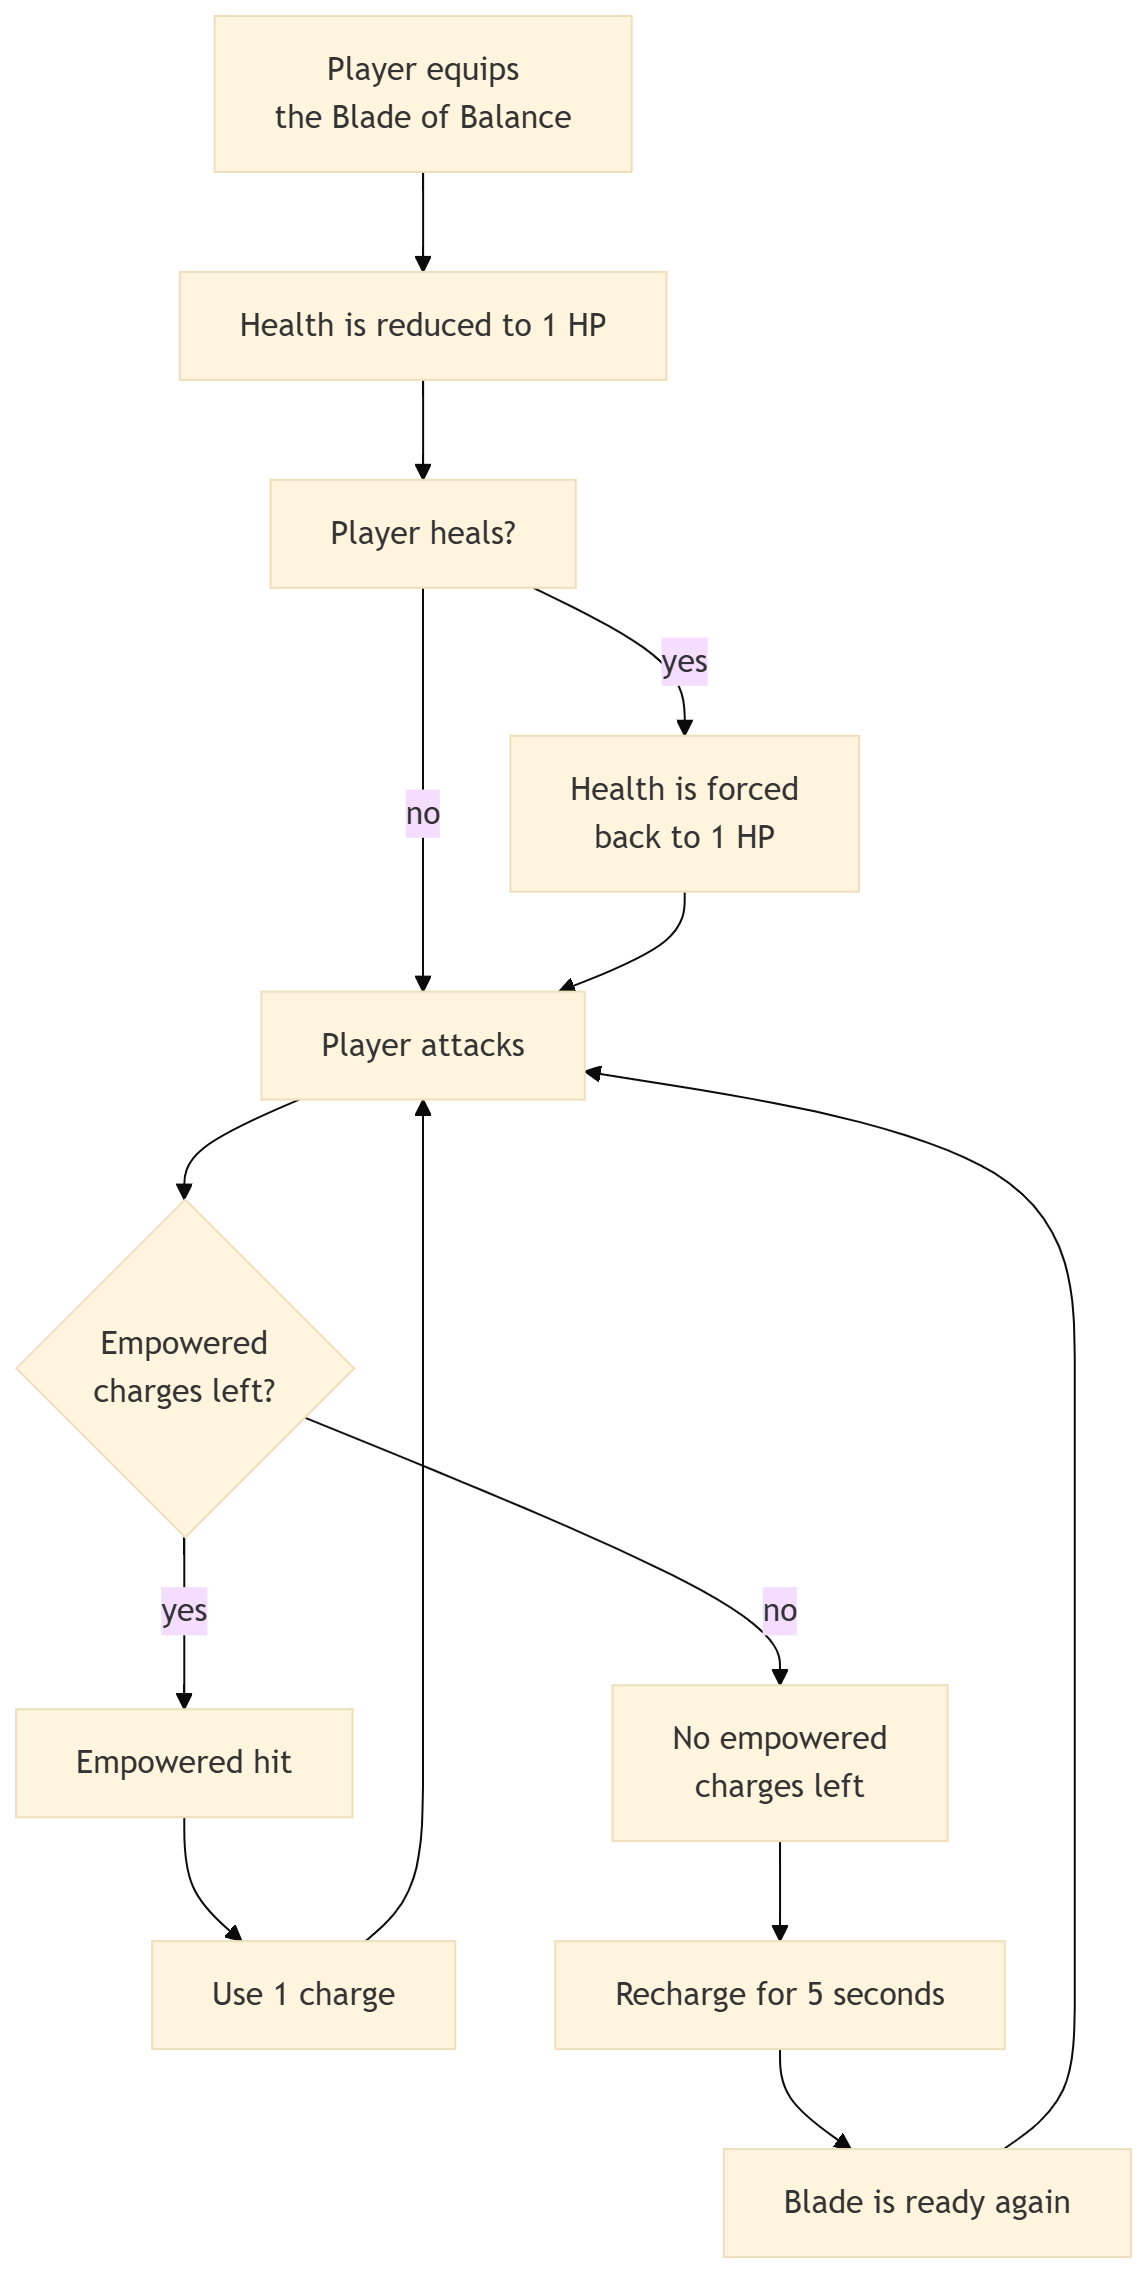
\includegraphics[height=0.55\textheight,keepaspectratio]{images/swordlogic}

    \small
    Figure: Logic of the Blade of Balance.
    While the blade is held during or after the trial,
    the player is kept at 1 HP.
    Its empowered attacks can only be used a limited number of times
    before a recharge phase begins.
\end{center}

The damage system adds a second limitation.
A permanently infinite-damage weapon removed too much tension,
so the Blade has three empowered hits before it must recharge for five seconds.
This creates short windows of power followed by forced weakness.
The player can kill almost anything,
but cannot attack endlessly.

Monster spawning supports this design.
The initial wave contains flying,
small,
normal,
and giant monsters,
plus a concentrated herd of rats.
The rat herd became important because small enemies are harder to control
when the player has only one hit point
and the Blade may be recharging.
A planned reinforcement system was disabled,
because spawning NPCs from inside a ticking system conflicted with Hytale's
entity store processing.
The initial wave remains,
but automatic reinforcements were removed for stability.

The Sacred Flower objective also had to be simplified.
Random terrain-based spawning was unreliable:
the flower could appear in the air,
underground,
inside grass,
too far away,
or at the wrong height.
The final version uses manually configured flower positions on a fixed map.
The positions are shuffled when the trial starts,
and the spawner tries them until a valid one works.


\subsection{Player Feedback}

The feedback layer makes the trial understandable and atmospheric.
Without dialogue,
UI,
objectives,
chat messages,
and sound effects,
the mod would still work mechanically,
but it would feel like a debug script:
a sword appears,
health changes,
monsters spawn,
and a flower has to be found.

The Goddess dialogue was difficult because Hytale's title display worked best
with one short line at a time.
My first version was too long and slowed the beginning of the trial down.
I rewrote it into shorter,
ritual-like title pages
and added a skip feature:
pressing the interaction key again while the Goddess is speaking
opens the offer UI immediately.
This keeps the atmosphere for the first interaction,
but makes repeated testing and replaying less frustrating.

Sound became part of the same feedback system.
Custom sound events were added for the Goddess voice
and for receiving the Blade of Balance.
The Goddess sound is calm and divine,
while the Blade sound is tense and eerie.
This contrast supports the uncertainty around the Goddess:
her words are gentle,
but her weapon feels dangerous.

The objective system was simplified for reliability.
I originally wanted it to update after the Sacred Flower was picked up,
but mid-trial objective updates did not behave reliably.
The final objective therefore gives the full instruction from the beginning:
find the Sacred Flower nearby and return it to the statue.
A compass marker was also planned,
but abandoned because it did not appear reliably.
Instead,
the flower itself became the guide through its purple glow.


\subsection{Cleanup Systems}

Cleanup became one of the most important parts of the plugin
because the trial temporarily changes the player,
the inventory,
and the world.
It gives special items,
places a flower block,
spawns monsters,
changes health behavior,
tracks objectives,
and stores trial state.
If any of these remain after death,
disconnect,
restart,
or failed testing,
the world quickly becomes polluted with leftover objects and broken states.

The final cleanup behavior is defensive.
On death,
the trial is failed,
the objective is cleared,
temporary items are removed,
Blade energy is cleared,
flower cleanup is attempted,
and monster cleanup is scheduled.
On join,
a delayed validation checks whether cleanup is pending
and removes leftover state where possible.
On server shutdown,
ongoing trials are marked as failed
so that cleanup can continue after restart.
For debugging,
\texttt{/trial reload} performs a stronger manual reset
by clearing trial items,
objectives,
flower positions,
health behavior,
and trial state.

Cleanup also separates failure from success.
If the player dies,
the trial resets and can be attempted again.
If the player completes the ritual,
the Goddess becomes whole,
the completed state is saved permanently,
and the player keeps the Blade of Balance as a reward.
In this way,
cleanup is not only technical maintenance.
It protects the story state of the mod.
